\documentclass[tikz,border=10pt]{standalone}
\usepackage{amsmath}
\usepackage{xcolor}

\begin{document}

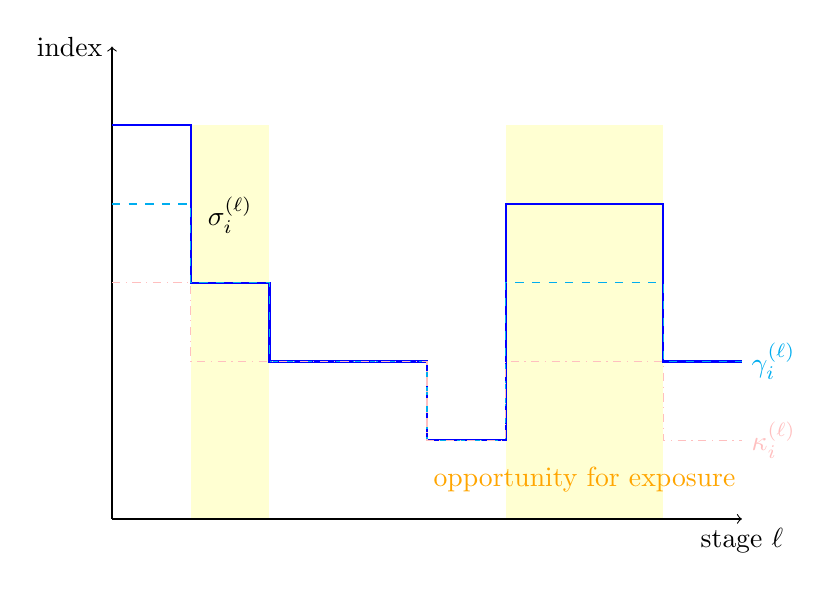
\begin{tikzpicture}

% Colors
\definecolor{lightyellow}{RGB}{255, 255, 210}
\definecolor{lightblue}{RGB}{102, 178, 255}
\definecolor{lightpink}{RGB}{255, 153, 204}
\definecolor{orange}{RGB}{255, 165, 0}

% Shaded regions
\fill[lightyellow] (1,0) rectangle (2,5);
\fill[lightyellow] (5,0) rectangle (7,5);

% Axes
\draw[->] (0,0) -- (8,0) node[below] {stage $\ell$};
\draw[->] (0,0) -- (0,6) node[left] {index};

% Horizontal lines
\draw[thick] (1,3) -- (2,3);
\draw[thick] (5,4) -- (7,4);

% Step functions
\draw[thick,blue] (0,5) -- (1,5) -- (1,3) -- (2,3) -- (2,2) -- (4,2) -- (4,1) -- (5,1) -- (5,4) -- (7,4) -- (7,2) -- (8,2);
\draw[dashed,cyan] (0,4) -- (1,4) -- (1,3) -- (2,3) -- (2,2) -- (4,2) -- (4,1) -- (5,1) -- (5,3) -- (7,3) -- (7,2) -- (8,2);
\draw[dash dot,pink] (0,3) -- (1,3) -- (1,2) -- (2,2) -- (2,2) -- (4,2) -- (4,1) -- (5,1) -- (5,2) -- (7,2) -- (7,1) -- (8,1);

% Labels
\node at (1.5,3.5) [above] {$\sigma_i^{(\ell)}$};
\node at (8,2) [right,cyan] {$\gamma_i^{(\ell)}$};
\node at (8,1) [right,pink] {$\kappa_i^{(\ell)}$};

% Opportunity for exposure
\node[orange] at (6,0.5) {opportunity for exposure};

\end{tikzpicture}

\end{document}